\chapter{Power management}
Il termine power management è stato usato nel corso degli anni per raggruppare problemi di diversa tipologia, ma che ruotano tutti attorno al concetto di energia.
Tra questi infatti si può includere:
\begin{itemize}
    \item Power management legata alla gestione della potenza assorbita,che si può a sua volta suddivisa in:
    \begin{itemize}
        \item Thermal Design Power, potenza termica massima che un componente può dissipare;
        \item Therm Design Current o Peak Current, legata alla massima corrente erogabile da alimentatori o dai pad dei chip; %todo: change
    \end{itemize}
    \item Thermal management, gestione temperatura dinamica o statica;
    \item Energy management, gestione della sostenibilità e del consumo di energia;
\end{itemize}

In questa tesi, si farà riferimento a questa parola per abbracciare tutti e tre i concetti che essa può rappresentare, portando così una visione olistica e più completa del problema.

Il contesto nel quale viene definito un Power Management è spesso un sistema di \emph{High-Performance Computing}, detto anche sistema HPC. Questi ultimi sono macchine computazionali composte da decine di centinaia di nodi interconnessi tra di loro da reti a bassa latenza e alta banda. L'insieme dei nodi, visto l'elevato numero di processori e agli acceleratori che hanno montato al loro interno offrono capacità computazioni che nei giorni nostri hanno raggiunto ordini del ExaFlops ($10^{18}$ operazioni di  Floating Point per secondo).
Con l'aumento della densità energetica unita alle notevoli prestazioni raggiunte, la potenza necessaria per alimentare questi sistemi sta superando la precedente soglia dei 20MWatt. Se poi si considera che la maggior parte della potenza fornita, viene convertita in calore, si deve prendere in considerazione anche i consumi necessaria per tenere raffreddati i sistemi. Infatti se non adeguati, le difficili condizioni in cui lavorano comportano grandi inefficienze in termini di energia, che si traducono anche in degradazioni di prestazioni computazionali. 
Considerando tutto, i centri che ospitano queste macchine necessitano di decine di MWatt di potenza per ogni exa-supercomputer che hanno in funzionamento. 
Ordini di grandezza di questo tipo non sono facilmente raggiungibili e anche quando lo sono, hanno costi estremamente elevati. 
%Inoltre i prezzi per garantire questi valori di Watt aumenta in modo non lineare.
Al fine di definire dei power budget, e utilizzare efficientemente la potenza richiesta si sono resi necessari strumenti situati su diversi livelli di astrazione. 
Sono nati così i primi concetti di Power Management, componenti per controllare l'utilizzo di energia utilizzando diverse strategie al fine di ridurre gli sprechi energetici e, allo stesso tempo, garantire un temperatura di funzionamento sicura.%Power Management può essere visto come un sistema composto sia da parti software che Hardware.
L'insieme dei componenti software e hardware che svolgono il compito di Power Management vanno a formare un power-stack in grado di gestire la potenza assorbita di macchine HPC.

\section{Stato dell'arte}
Un Power-Stack deve gestire e monitorare la potenza assorbita, le frequenze e le temperature di processori all'interno dei sistemi. Questo deve poter essere fatto anche a diversi livelli come intero sistema,
\setlength{\intextsep}{1pt} % Adjust the vertical space here (5pt in this example)
\begin{wrapfigure}{r}{0.4\textwidth}
    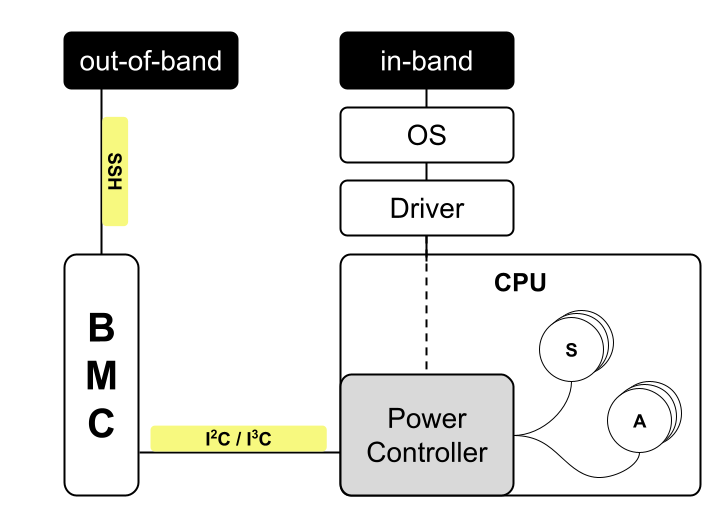
\includegraphics[width=0.4\textwidth]{img/SoA.png}
    \centering
    \caption{Differenza tra le due interfacce} 
    \label{fig:SoAinoutband}
\end{wrapfigure}
singoli nodi e singoli elementi all'interno dei nodi. E' quindi necessario poter accedere agli attuatori e sensori presenti nei core sia in modo diretto che da "remoto". Normalmente sono rese disponibili due tipi di interfacce:
Nella figura \ref{fig:SoAinoutband} viene schematizzata la differenza tra le due interfacce disponibili. 
\begin{itemize}
    \item in-band
    \item out-of-band
\end{itemize}
Nella figura \ref{fig:SoAinoutband} viene schematizzato l'accesso ai dispositivi hardware che si occupano della gestione del power management su sistemi HPC. Sarebbe in realtà possibile accedere a questi componenti anche tramite altri meccanismi specifici, ad esempio la mappatura in memoria condivisa, tuttavia a causa della loro natura altamente specializzata, tali approcci non saranno inclusi nell'ambito di questa tesi.

% I servizi in-band vengono forniti alle applicazioni e ai sistemi operativi in esecuzione negli elementi di elaborazione del chip e sono composti da: (i) governor dedicati alla potenza e telemetria correlata alla potenza a livello di sistema operativo; (ii) un'interfaccia dedicata per consentire alle applicazioni e ai tempi di esecuzione del modello di programmazione di specificare suggerimenti e prescrizioni per la gestione della potenza; (iii) un'interfaccia dedicata al Sistema e alla Gestione delle Risorse per supportare il capping della potenza a livello di CPU e nodo, nonché per gestire il compromesso tra Throughput ed Efficienza Energetica. I servizi out-of-band vengono forniti all'amministratore di sistema e agli strumenti di gestione del sistema tramite il Controller di Gestione della Scheda (BMC). Questi servizi consistono nella telemetria di potenza out-of-band, nel capping di potenza a livello di sistema e nella affidabilità e assistenza.

% (ii) off-chip ai Moduli Regolatori di Tensione (VRM) che alimentano il chip, gli altri componenti a bordo e il Controller di Gestione della Scheda (BMC).

\subsection{Servizi in-band} %TODO da sistemare

I servizi in-band accedono alle risorse hardware tramite codice che esegue sul processore stesso. Questi sono resi possibili da infrastrutture come CPUfreq o RAPL che tramite dei driver, espongono a livello utente tramite  sistema operativo, le manopole per gestire e monitorare frequenze e informazioni della cpu. Queste ultime possono essere gestite in modo manuale, in automatico in base al carico di sistema oppure in risposta ad eventi ACPI. Una volta scelti i driver come \emph{ACPI CPUfreq driver} e \emph{Intel P-state} è possibile scegliere tra diversi governors (o governatori) ognuno che agisce con delle policy specifiche.
Per esempio in \emph{CPUfreq} fornisce diversi governors per soddisfare diversi tipi di situazioni, come:
\begin{itemize}
    \item performance: forza la CPU ad eseguire alla frequenza massima disponibile;
    \item powersave: forza quella minima;
    \item ondemand: comportamento dinamico in base all'utilizzo di sistema;
    \item userspace: permette ai selezionati user-space di impostare la frequenza; 
    \item conservative: come ondemand ma con più inerzia al cambiamento;
\end{itemize}

\begin{figure}[H]
    \centering
    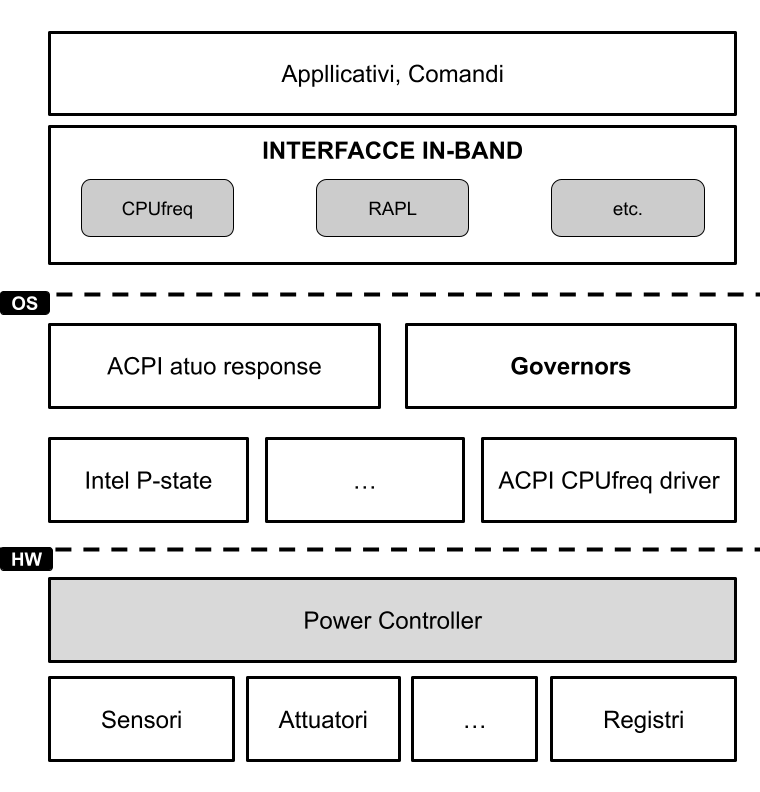
\includegraphics[width=0.9\textwidth]{img/in-band.png}
    \caption{Struttura interfacce in-band: divise su più livelli tra cui Sistema Operativo (SO) e Hardware (HW) } 
    \label{fig:inband}
\end{figure}

Il vantaggio di usare queste interfacce è che permettono di operare in \gls{Real-Time} ed in modo dinamico. I lati negativi invece risiedono nelle stesse peculiarità di questi strumenti, ovvero che possono ottenere solo le informazioni dei core sui quali i richiedenti vengono eseguiti. 

% E' reso possibili tramite degli specifici driver (intel\_pstate) che comunicano con i componenti hardware sul chip. Diversamente \textbf{Intel Power Governors} utilizza le interfacce proprietarie (RAPL) con cui monitora potenza ed energia a livello di sistema.
% Entrambi questi strumenti hanno necessità di componenti Hardware dedicati come i power knob (manopole per la gestione della potenza) e sensori che permettono di monitorare temperature e tensioni.
% I servizi in-band sono molto flessibili e permetto di operare in real-time ed in modo dinamico. Infatti interagendo con l' Hardware e passando tramite il sistema operativo, sono necessari semplici chiamate e comandi per controllare questi strumenti.

%TODO: schema power governors e power controller

\subsection{Servizi out-of-band}
Contrariamente alle interfacce in-band, le out-of-band fanno utlizzo di \emph{sidechannels} ovvero canali di accesso alternativi per ottenere le informazioni richieste. Questo meccanismo permette di accedere ad informazioni da processi esterni dal processore del quale si vuole impostare o reperire dei dati. Per di più questo permette di monitorare i componenti anche quando ci sono errori ed eccezioni che normalmente bloccherebbe il workflow. Un componente tra i più famosi che svolge questa funzione è il Baseboard Management Controllers (BMC), solitamente un microcontrollore animato da sistemi embedded linux, e accessibile tramite un canale separato (solitamente provvisto di una propria interfaccia di rete e/o bus specifici). Il suo principale scopo è quello di monitorare in modo dettagliato lo stato di tensioni, temperature, ventole e prestazioni dei processori e fornire contemporaneamente servizi di power capping sia a livello di sistema (non possibile tramite le interfacce in-band) che di singoli processori.
Recentemente alcuni produttori di BMC introducono anche dispositivi FPGA da affiancare al BMC per aumentarne la flessibilità e le prestazioni.
%TODO: se vuoi spiegare esempi di bmc come opencms e aspeed astd2600
% HDEEM Estende bmc con FPGA che legge le potenze HFrequency
% \vfil
\begin{figure}[H]
    \centering
    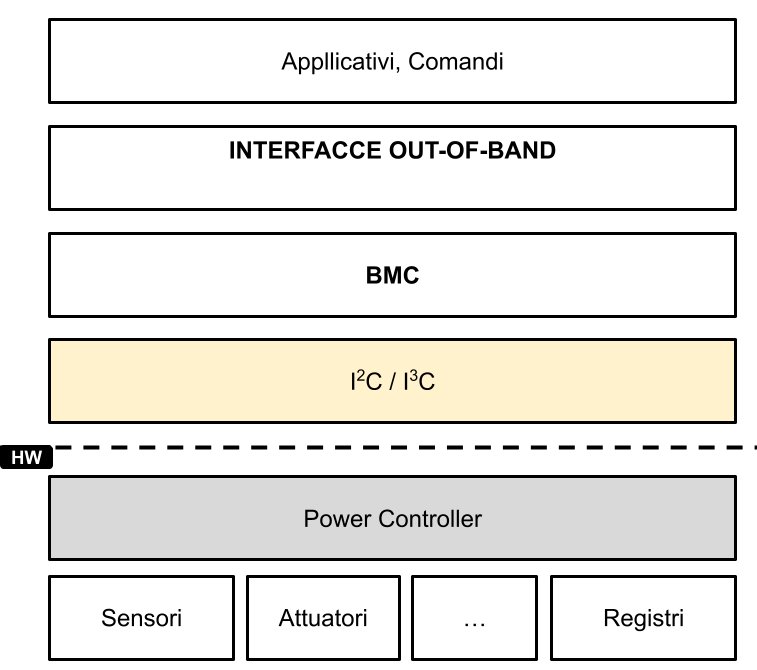
\includegraphics[width=0.9\textwidth]{img/out-of-band.png}
    \caption{Struttura interfacce out-of-band} 
    \label{fig:inband}
\end{figure}


\section{Interfacce di alto livello}
Nel corso degli anni con l'obbiettivo di ottimizzare e automatizzare l'interazione con questi meccanismi hardware sono stati sviluppati diversi software di più alto livello che utilizzano sia interfacce in band che interfacce out of band. Si possono ricordare i più famosi: \emph{Variorum} (LLNL), \emph{GEOPM} (Intel)\cite{GEOPM}, e \emph{HDEEM} (Atos)\cite{HDEEM}. Tutti questi rappresentano però un tentativo di fornire una soluzione ad un sottoinsieme di problemi per la gestione dell'energia o potenza, piuttosto che ad un software con visione globale di Power Management per sistemi di calcolo ad alte prestazioni. %MANCANZA DI VISIONE GLOBALE!!!


\section{Modello di power stack} %Componenti power stack
Con Power-Stack si intende un insieme di applicazioni software che cooperando riescono a fornire ad applicazioni, utenti e amministratori gli strumenti per un servizio di Power Management. Una volta definito il problema, e i componenti che possono essere utilizzati, è possibile definire un modello di interazione e responsabilità dei vari attori. Di seguito vengono riportati quelli che sono i ruoli necessari al fine di coordinare un sistema HPC dall'allocazione di un applicativo, fino alla gestione delle tensioni. 
\begin{itemize}
    \item Workflow engine (WE)
    \item System Manager (SM)
    \item Job Manager (JM)
    \item Resource Manager (RM)
    \item Node Manager (NM)
    \item Monitor (M)
\end{itemize}
%TODO add an example of each component
%TODO aggiungi i tipi di informazioni che si scambiano, per facilitare nel modello la realizzaizone

\subsection{Workflow engine}
Il workflow rappresenta un flusso di lavoro composto da diversi task che deve essere svolto per risolvere un determinato problema. Il workflow engine si occupa di analizzare le dipendenze e le richieste di risorse di ogni workflow e decide dinamicamente come dividerlo negli specifici jobs che verranno assegnati al system-manager. %Si occupa quindi di analizzare ed assegnare i diversi task a chi poi va ad eseguirli.

\subsection{System Manager}
Il System Manager dopo aver ricevuto come input un insieme di jobs li schedula all'interno del sistema, e in modo indicativo decide quando schedulare ogni job, su quale nodo, e con quale power budget. In contemporanea una parte chiamata System Power Manager %o TODO:managment?
si occupa di comunicare con tutti i Node Manager all'interno del sistema, per impostare eventuali limiti di potenza. Questi ultimi vengono solitamente impostati manualmente dagli amministratori di sistema, oppure in modo automatico comunicando con gli altri attori, come monitor e NM. Una volta fissati i limiti, vengono monitorati i dati relativi a potenza ed energia, e controlla di conseguenza i budget, e la \emph{user-fairness}.

\subsection{Job schedulers}
Il job scheduler ha il compito di assegnare e condividere le risorse computazionali e fisiche del sistema HPC, ai vari utenti che lo utilizzano. In particolare la serie di compiti che si trova a svolgere è il seguente:
\begin{enumerate}
    \item L'utente schedula i jobs da svolgere in una o più code, definite dallo scheduler.
    \item Il Job scheduler esamina tutte le code e i job in esse contenute, e decide dinamicamente, quale sarà l'ordine di esecuzione, e il tempo massimo in cui viene assegnata una risorsa.
\end{enumerate}
Generalmente si cerca di ottimizzare alcune caratteristiche come il tempo di utilizzo del sistema oppure l'accesso veloce alle risorse per alcuni sottoinsiemi di jobs. Inoltre le code definite, possono avere diverse priorità o può essere ristretto l'accesso a soli alcuni utenti. I job scheduler possono condividere un nodo anche con più utenti contemporaneamente, in base all'utilizzo che devono farne. Per farlo il nodo viene allocato e diviso in partizioni virtuali, che vengo "sciolte" una volta finiti i job in esecuzione. Questo permette di utilizzare al massimo i componenti messi a disposizione dal sistema HPC.

\subsection{Resource Manager}
Per riuscire a svolgere questo lavoro il Job Scheduler interagisce con uno o più \textbf{Resource Manager}. Questi sono software che hanno il privilegio di gestire le risorse di un centro di calcolo. Queste risorse includono diversi componenti:
\begin{itemize}
    \item Nodi
    \item Processori
    \item Memorie
    \item Dischi
    \item Canali di comunicazione (compresi quelli di I/O)
    \item Interfacce di rete 
\end{itemize}
Per esempio quando un Job Scheduler deve eseguire un job, richiede al RM di allocare core, memorie, dischi e risorse di rete in linea con quanto il job ha necessita di essere eseguito.

Infine in alcuni casi il RM è anche responsabile di gestire elettricità e raffreddamento dei centri di calcolo.


\subsection{Job Manager}
Lo scopo del job manager è quello di effettuare ottimizzazioni job-centriche considerando le prestazioni di ogni applicazioni, il suo utilizzo di risorse, la sua fase e qualsiasi interazione dettata da ogni workflow in cui è presente. In breve il job manager decide i target delle manopole del Power Management, come (i) CPU power cap, (ii) CPU clock frequency oltre ad eseguire ottimizzazione del codice.

\subsection{Node Manager}
Il node manager fornisce accesso ai controlli e monitoraggio hardware a livello del nodo. Volendo permette anche di definire delle policy di power management. Ha infine lo scopo di preservare integrità, sicurezza del nodo sia in termini informatici che fisici.

\subsection{Monitor}

Il monitor è responsabile di collezionare tutte le metriche in-band e out-of-band che riguardando prestazioni, utilizzo e stato delle risorse, potenza ed energia.
Tutto questo deve essere fatto con il minor impatto possibile sul sistema dove sta agendo, collezionando, aggregando e analizzando le metriche e dove necessario, scambiandole ad altri attori. A sua volta il \emph{Monitor} è scomponibile in tre sotto-moduli:
\begin{itemize}
    \item Gestione Firma che genera una firma che identifica univocamente il job; 
    \item Estimatore che valuta le proprità dei job o dello stato del sistema usando la firma generata precedentemente;
    \item Dashboard che fornisce le funzionalità da mostrare agli sviluppatori.
\end{itemize}


Per concludere viene mostrato uno schema in figura \ref{fig:powerstackscheme} che vuole mostrare la gerarchia e le possibili interazioni tra i vari attori.
\begin{figure}[H]
    \centering
    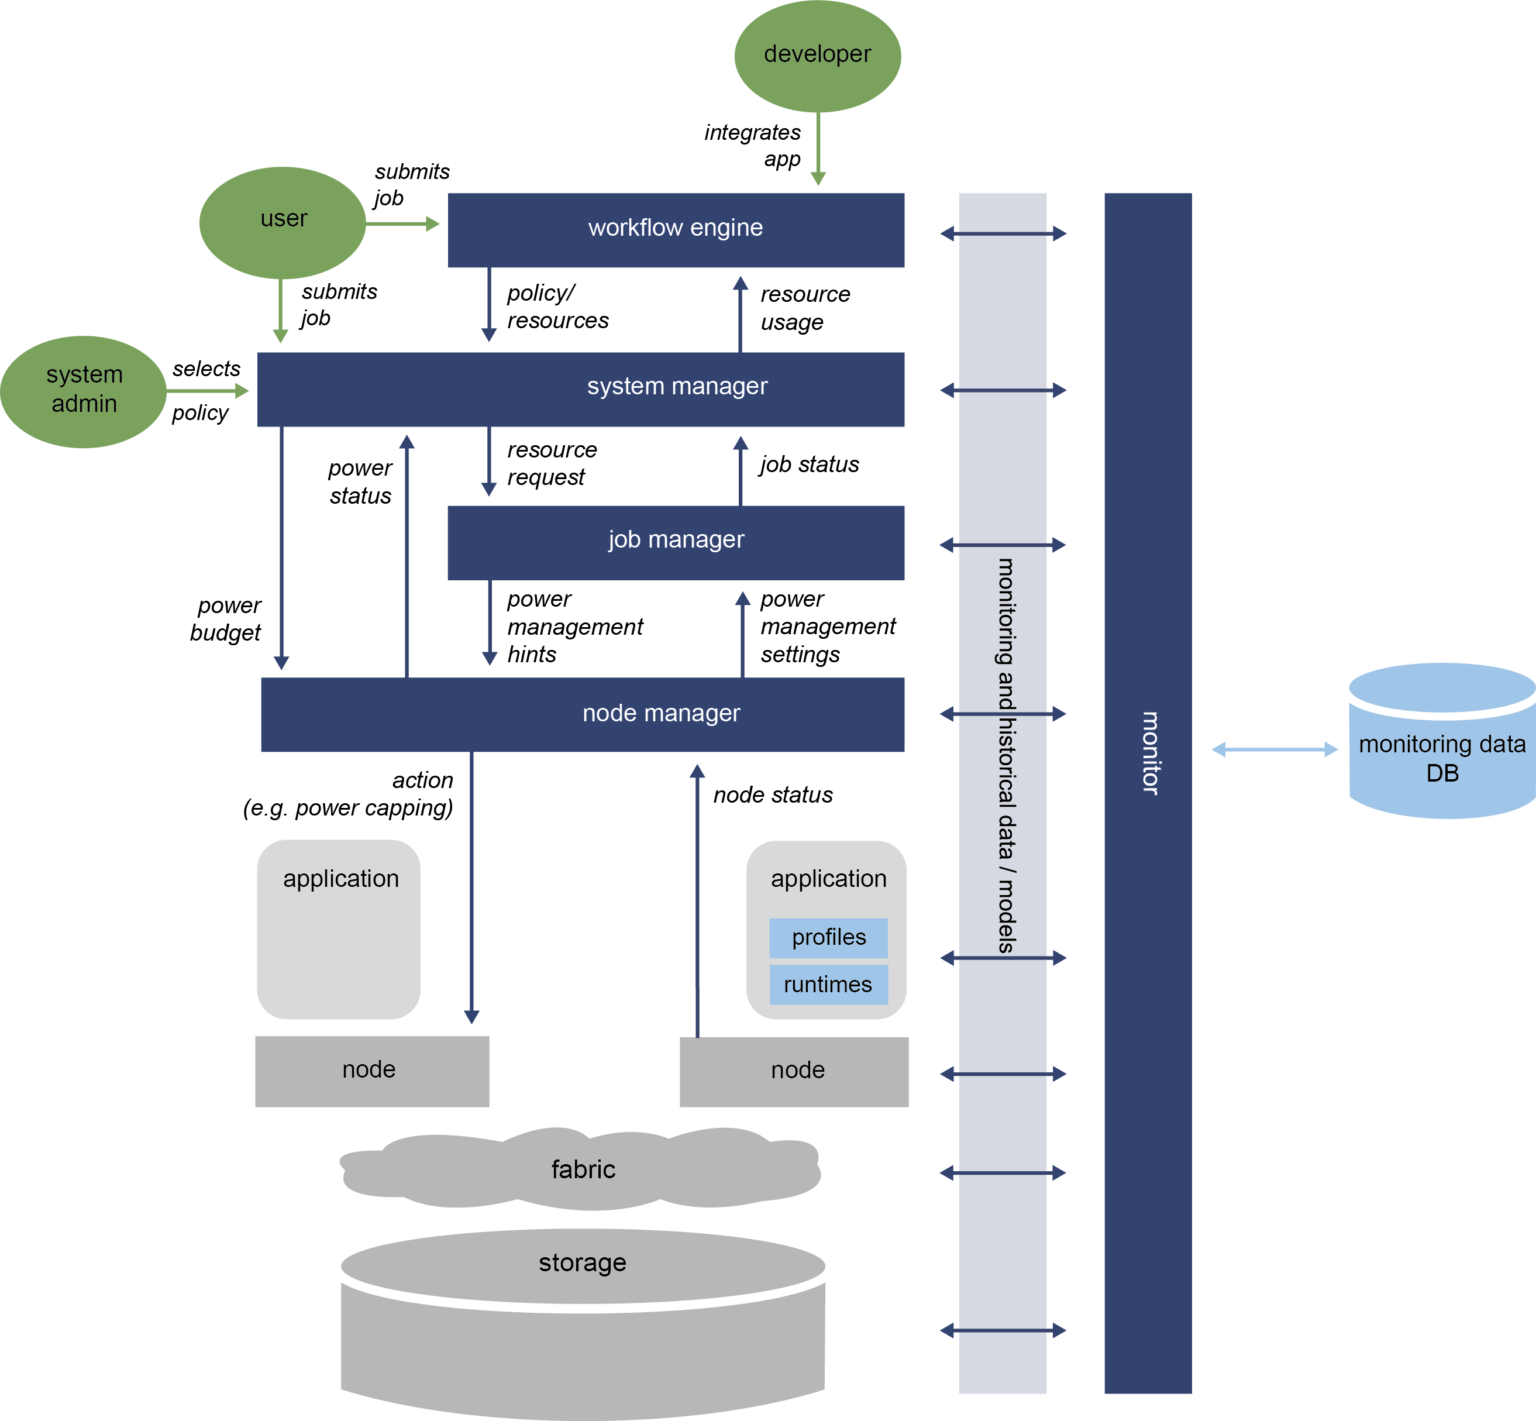
\includegraphics[width=\textwidth]{img/REGALE-Architecture-1536x1421.png}
    \caption{Modello di power stack} 
    \label{fig:powerstackscheme}
\end{figure}

% TODO:
% To ask andrea:
% Quali di questi componenti sono out-in band?